\chapter{系统架构设计}

\section{概述}

无感知人脸识别系统的架构设计主要分为三部分:数据处理流程、设备网络拓扑结构和系统逻辑架构。其中,数据处理流程主要描述系统中的数据存储结构,数据格式和数据流动情况。设备网络拓扑结构主要描述系统中所有机器的物理部署特征,网络拓扑等。系统逻辑架构主要描述系统实现代码中所有的模块和组件,以及不同模块组件之间的交互与职能分配。

\section{数据处理流程}

无感知人脸识别系统的数据处理流程如图\ref{fig:chap5:data}所示:

\begin{figure}[!htp]
	\centering
	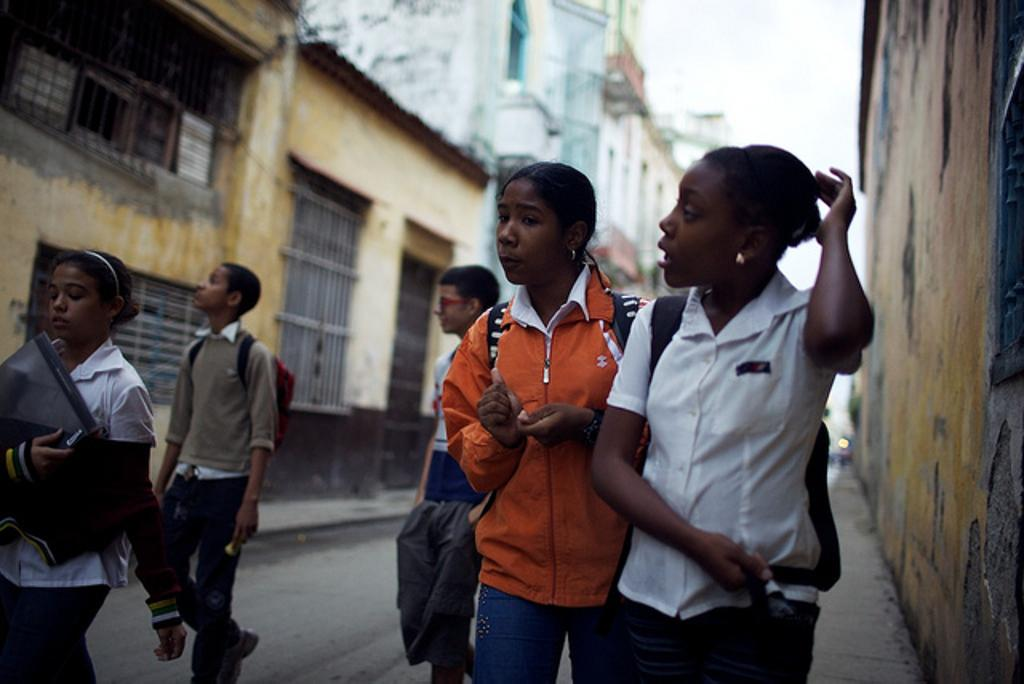
\includegraphics[height=1.7cm]{chap5/1.jpg}
	\bicaption[系统数据处理流程图]
	{系统数据处理流程图}
	{System data architecture}
	\label{fig:chap5:data}
\end{figure}

图\ref{fig:chap5:data}中标注为1的部分表示视频流的帧截取过程;标注2的部分代表了人脸区域检测的过程;标注3的部分代表了人脸识别的过程;标注4的部分代表了人脸匹配的过程。

最先进入系统的是由摄像设备和嵌入式设备获取的视频流数据,这部分数据在本地进行帧截取操作后会将获得的图片上传到图片队列中。图片队列是一个被服务器维护的优先级队列,其长度根据系统的需求和服务器的性能确定。每接收到一张新的图片时,首先检查队列是否已满。如果队列已满,则将该图片丢弃,并向用户发送服务器繁忙的信息。如果队列未满,则根据该图片的优先级将该图片插入到队列中。队列中的每张图片都应有唯一的标记,以表明这张图片的发送源。

进行人脸检测时,每次从图片队列的前端取出一张图片进行检测,检测完成后根据图片标记将得到的人脸区域做好标记插入到人脸队列中。如果人脸队列已满,则将带标记的人脸区域存储在服务器中的特定硬盘区域。当人脸队列有空余位置时,从该硬盘区域中读取存储的内容加入人脸队列的尾部,并删除硬盘中的相应内容。

进行人脸识别时,每次从人脸队列的前端取出批尺寸大小的人脸图像及其标记加载到人脸识别模块中,得到批尺寸大小的特征向量及标记。接着将这些特征向量及其标记发送到人脸数据库中进行匹配。由于不同的请求之间没有数据依赖性,匹配模块的可以在高并发量的情况下运行,得到匹配的身份信息与每条信息的初始标记。

最后,根据每条身份信息的标记,将某一用户请求的所有身份信息返回给用户。

\section{设备网络拓扑结构}

无感知人脸识别系统的设备网络拓扑结构如图\ref{fig:chap5:phy}所示:

\begin{figure}[!htp]
	\centering
	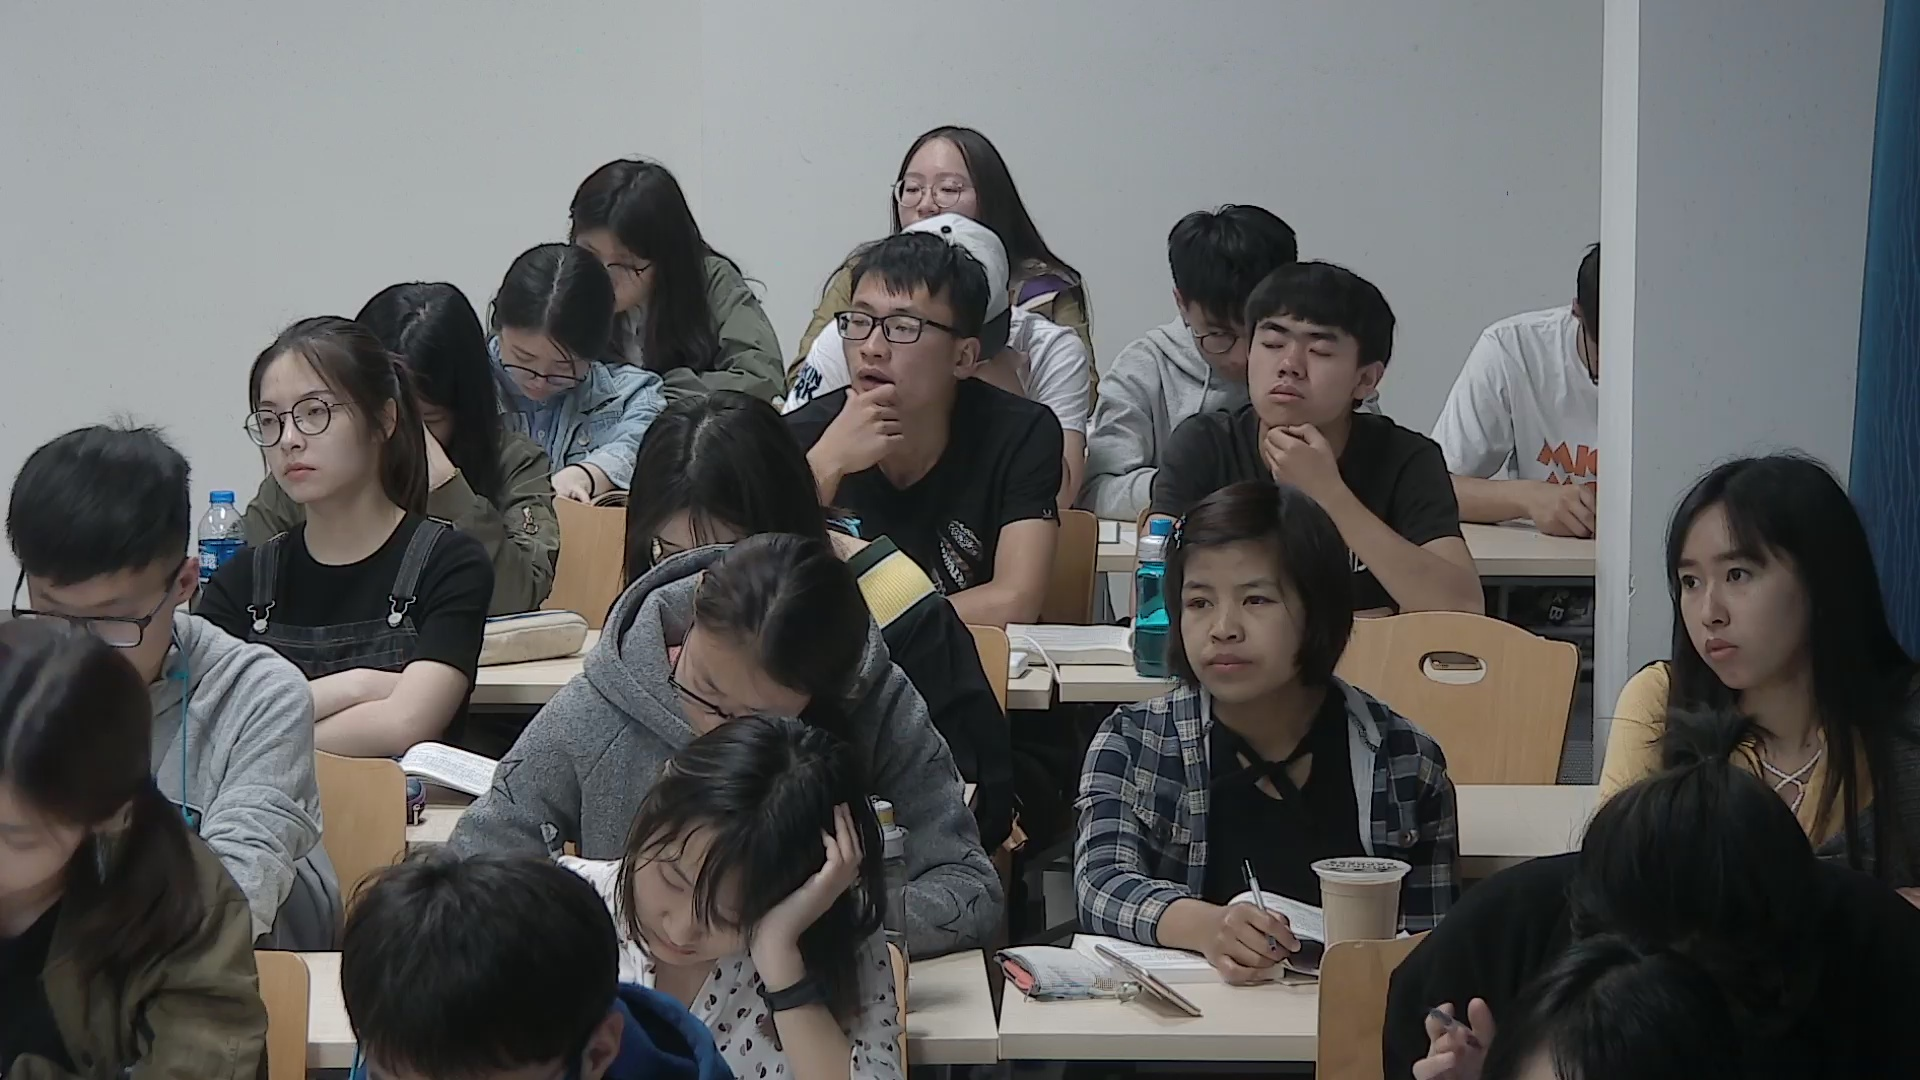
\includegraphics[height=4cm]{chap5/2.jpg}
	\bicaption[系统设备网络拓扑结构图]
	{系统设备网络拓扑结构图}
	{System physical architecture}
	\label{fig:chap5:phy}
\end{figure}

图\ref{fig:chap5:phy}中的标注1的部分表示摄像设备与GPU服务器集群之间通过有线网络连接,数据从摄像设备传输到GPU服务器集群;标注2表示嵌入式设备与GPU服务器集群之间通过无线网络连接,数据从嵌入式设备传输到GPU服务器集群;标注3表示GPU服务器集群与人脸数据库之间通过内部的有线网络连接;标注4表示人脸数据库与交互服务器通过内部的有线网络连接。

其中,人脸检测模块和人脸识别模块部署在GPU服务器集群中,人脸匹配模块部署在人脸数据库中。交互服务器负责分析匹配结果,并将分析后的到的信息发送到相应的用户设备中。

在系统的实际部署中,由于摄像设备和嵌入式设备的输入众多,网络拓扑结构会更为复杂,网络中很可能需要增加一些中间节点。如果GPU服务器集群不在本地而在云端,则整个网络传输就无法在一个局域网内进行。此时则需要考虑网络带宽对数据传输的影响。如果网络带宽不足,可会影响获取到的图片的传输速度,进而影响总体的识别速度。同时,如果GPU服务器集群和人脸数据库之间的传输需要经过公有网络,则考虑网络带宽的同时还需要考虑传输安全的问题。


\section{系统逻辑架构}

无感知人脸识别系统的系统逻辑架构如图\ref{fig:chap5:logic}所示:

\begin{figure}[!htp]
	\centering
	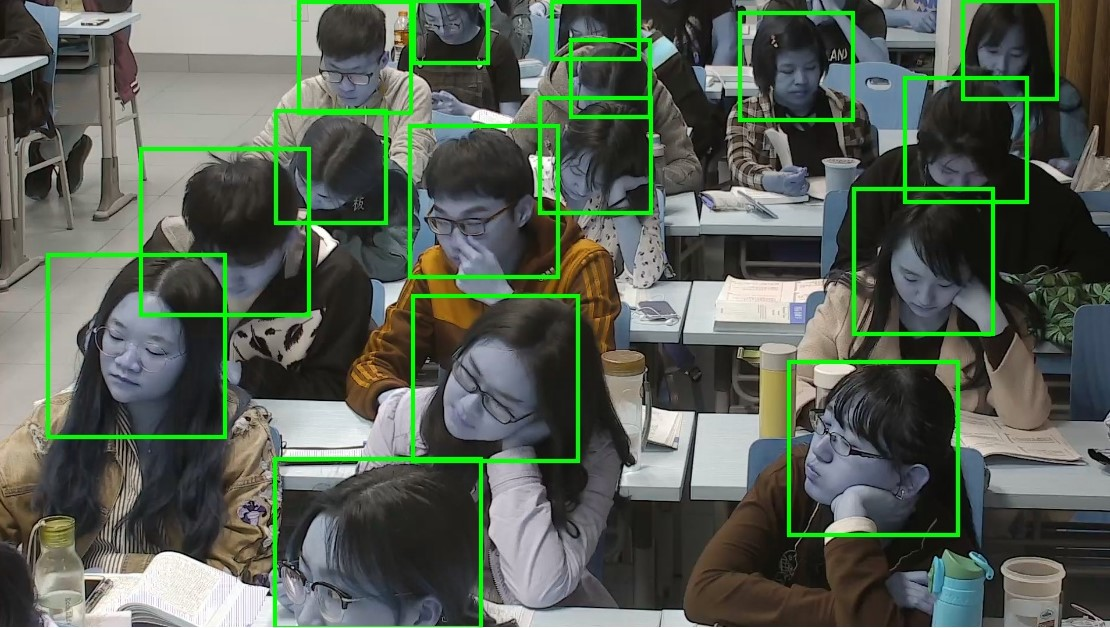
\includegraphics[height=2.5cm]{chap5/3.jpg}
	\bicaption[系统系统逻辑架构图]
	{系统系统逻辑架构图}
	{System logical architecture}
	\label{fig:chap5:logic}
\end{figure}

图\ref{fig:chap5:logic}中标注为1的部分为GPU服务器集群的负载均衡模块;标注为2的部分为使用Docker封装的人脸检测和人脸识别模块;标注为3的部分为人脸数据库服务器的负载均衡模块。

图像获取模块共有两种实现,一种部署到连接摄像设备的盒子中,另一种部署在嵌入式设备上。两种实现的功能都时从视频流中截取图像信息。根据实际需要,截取信息的操作可以是定时自发执行的,也可以是由用户或者服务器请求执行的。

通过第三章的对比,经过CFDDB的测试,SSH检测器\cite{najibi2017ssh}是目前唯一符合我们系统人脸检测需求的人脸检测器。因此,人脸检测模块中的算法优先选择SSH检测器。部署时需要考虑每一个SSH检测器需要的显存空间以最大化利用GPU服务器集群中的资源。如果未来有更优的算法,可以直接将其模块化,实现需要的接口后进行替换,而无需重写整个系统。

通过第四章的叙述,InsightFace\cite{deng2018arcface}符合我们系统的要求,因此将其封装为人脸识别模块。一个较好的系统设计是将人脸检测模块和人脸识别模块使用同一个Docker容器封装,外部程序通过使用GRPC框架调用容器内部的程序进而进行检测和识别。这样当算法有更新时,可以将更新完的Docker容器重新部署,加速部署的过程,减少服务器的停机时间。

如果人脸检测或人脸识别的算法使用了TensorFlow实现,可以使用TFserving进行封装。使得算法和模型的更新与新旧版本的管理变得更加便捷。

如果同时间有大量的匹配请求,在匹配模块之前的负载均衡模块也必不可缺。如果实际中人脸数据库较小,匹配模块内部可以采用线性搜索的方法。而如果数据库非常大,则可以使用近似搜索的算法加快搜索的效率。



